\chapter{Design of the RARS Mobile Robot}
\label{ch_3:Design}


Most of the mobile robots presented in literature use differential wheel drive  with passive castor as in \cite{saha1989kinematics}, \cite{yamamoto1992coordinating} and \cite{rajendran2004}. The other  common methods for locomotion of mobile robots are the omnidirectional wheels  \cite{pin1994new} and \cite{salih2006designing}, and tracked wheel system \cite{suthakorn2009design} and \cite{guarnieri2004development}. According  to  Nagatani \cite{nagatani2000improvement},  a  vehicle  with  Mecanum  wheels  is  susceptible  to slippage and same is the case for tracked vehicle, which are inherently skid steered. The slippage of the wheels prevents the most popular dead-reckoning method using rotary shaft  encoders   from  being  performed  well.

The major design objective for the  mobile manipulator at hand  was to make it fault tolerant to single actuator failure. This was important as  the mobile manipulator was to move in an environment where human access is prohibited. With the fault tolerant design it could be assured that the mobile manipulator can be extracted from the restricted zone even in case  one of its the actuator fails. 

 The proposed design combines differential drive for the two rear wheels and  motorized Davis mechanism for steering the front two passive wheels. This makes the system both Redundant Actuated in traction and Redundantly Steered (RARS). The proposed system has only 3 actuators as compared other redundant wheeled mobile robots which are having minimum 4 actuators.  
 
 In the literature, most common redundantly  actuated system are based on ether powered caster wheels (PCW) or omnidirectional wheels. One of the first mobile platform the CMU Rover \cite{moravec1982cmu, moravec1983stanford},  was a PCW based system.  Other PCW based robots are presented in \cite{oetomo2008singularity}, \cite{chung2010design}, \cite{li2006wheel} and \cite{park2002optimal}.   Mobile robots discussed in \cite{muir1987kinematic}, \cite{yi2002kinematics} and  \cite{saha1995design} are redundantly actuated systems based on omnidirectional wheels.  The RARS design scores over the omnidirectional wheels based system in terms of lesser number  of moving parts thus increasing its reliability. Because each omni wheel is made of multiple rollers. Moreover in industrial environment debris can clog the rollers and alter the friction characteristics of the wheels as shown in \cite{carlson2005ugvs}. 
   The PCW system has issues with singular configuration and wheel locking up the drive system due to improper coordination between steering actuators as discussed in \cite{oetomo2008singularity} and \cite{low2005kinematic}. Moreover, due to changing orientation of all wheels it becomes difficult for the operate to negotiate obstacles when operated in teleoperation mode.

This chapter   discusses kinematic topology and  the  design methodology of the RARS mobile manipulator. The advantage of  Davis steering mechanism is highlighted over castor wheels  or other steering methods. The actuator sizing and stability analysis of the RARS mobile robot is also presented.    
\section{Design Overview}
 The objective of a  mobile robot under consideration is to navigate inside the cyclotron vault and collect radiation intensity data at all the required points decided by the operator. Data is to be collected not only at different planer locations of the floor but also at varying height from the floor. To cater to this operational requirement, a mobile platform with a vertically extendable manipulating arm was developed. Together, they are   referred henceforth as "mobile manipulator" or simply "mobile platform". The 3-D model of the mobile-manipulator with its major subsystems are shown in Figure \ref{fig:robo3Dmodel}, whereas  and the actual   system  is shown in Figure  \ref{fig:roboActual}. 

 The environmental condition required that the vehicle be either  autonomous or teleoperated. To keep the complexity low, it was decided to have wireless teleoperated   navigation and control. This gives an  operator full flexibility to drive  and control the system from a remote station  using  visual  feedback provided from the on-board camera. The key parameters of the mobile manipulator are listed in  Table \ref{tb:specifications}.

\begin{figure}[h]
	\centering
	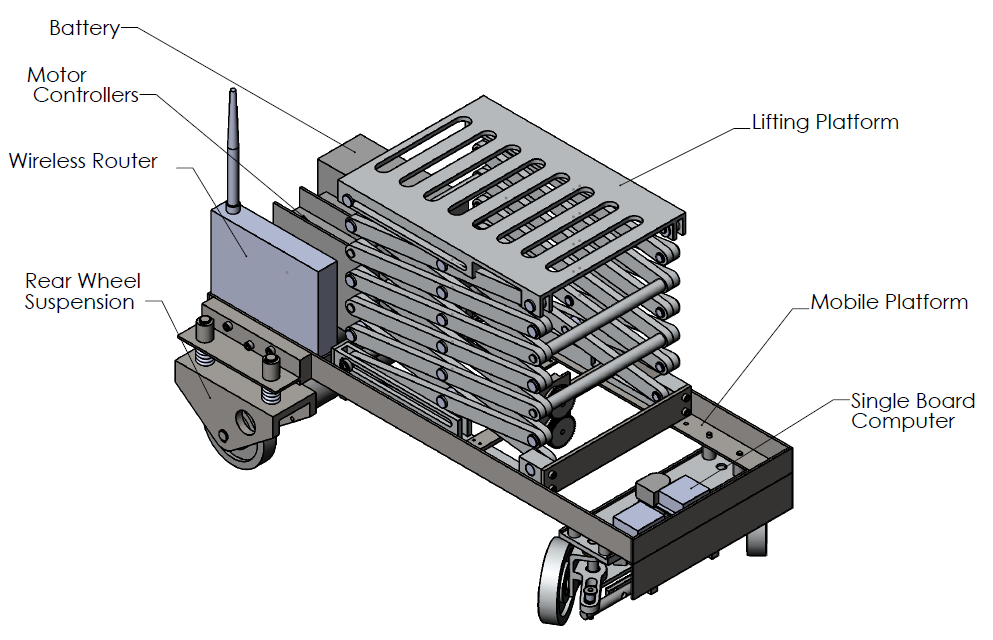
\includegraphics[width=\linewidth,keepaspectratio]{Chapter3/fig/robo3Dmodel}
	\captionof{figure}{3-D Model of the mobile manipulator}
	\label{fig:robo3Dmodel}
\end{figure}
\begin{figure}[h]
 		\centering
		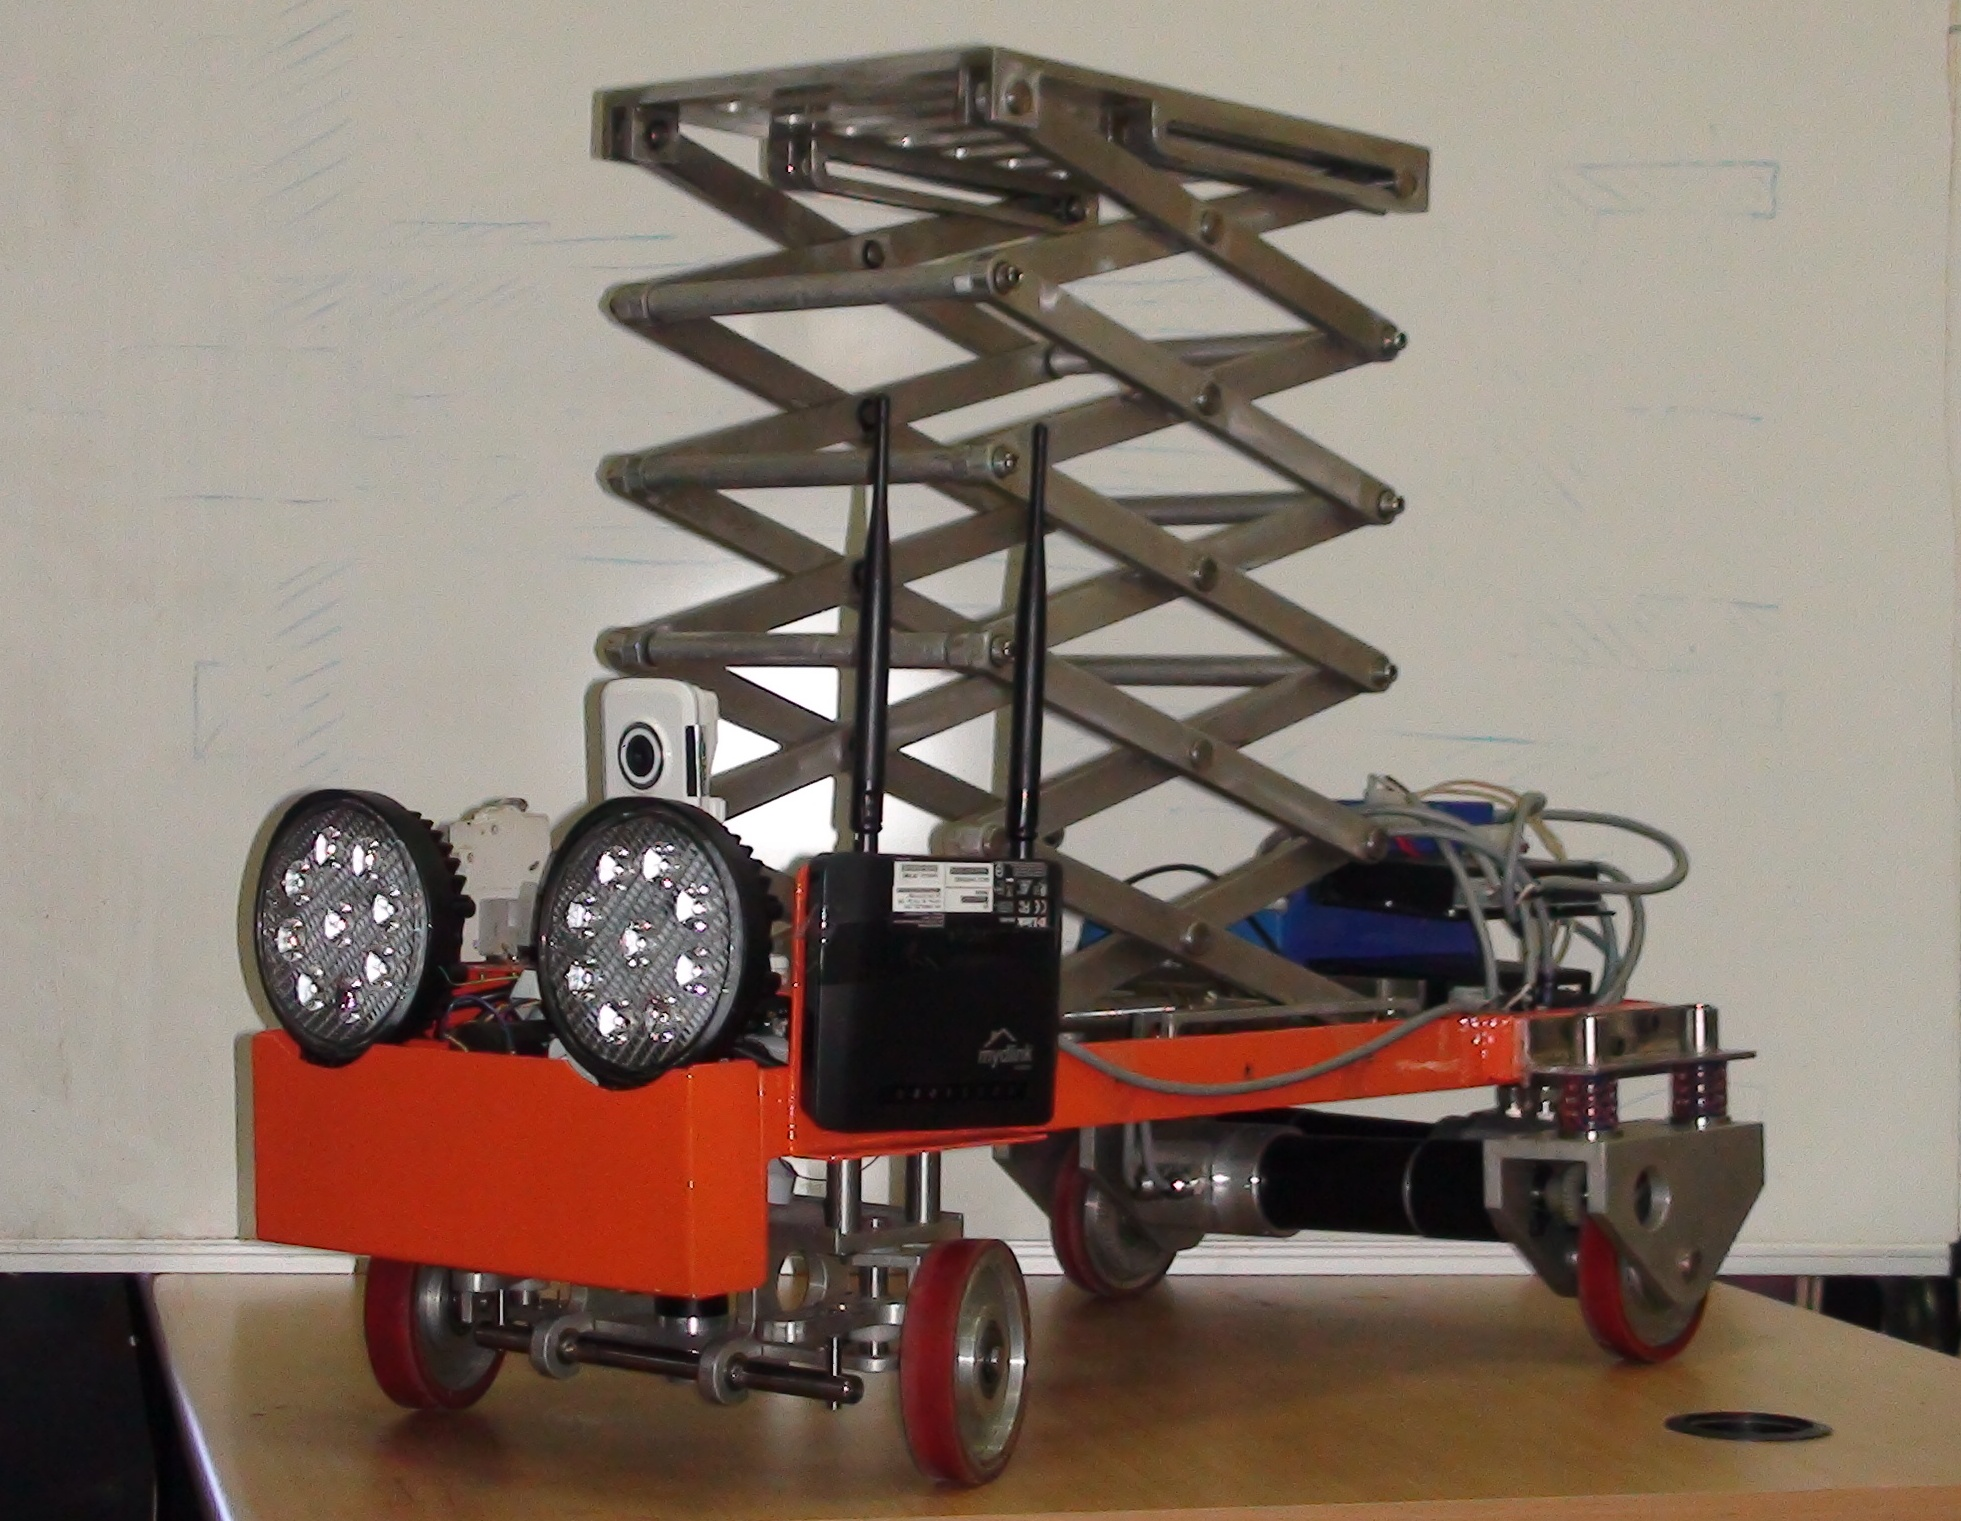
\includegraphics[width=.8\linewidth,keepaspectratio]{Chapter3/fig/roboActual}
		\captionof{figure}{Photograph of the actual system}
		\label{fig:roboActual}
\end{figure}

% \begin{figure}
% 	\centering
% 	\begin{minipage}{.5\textwidth}
% 		\centering
% 		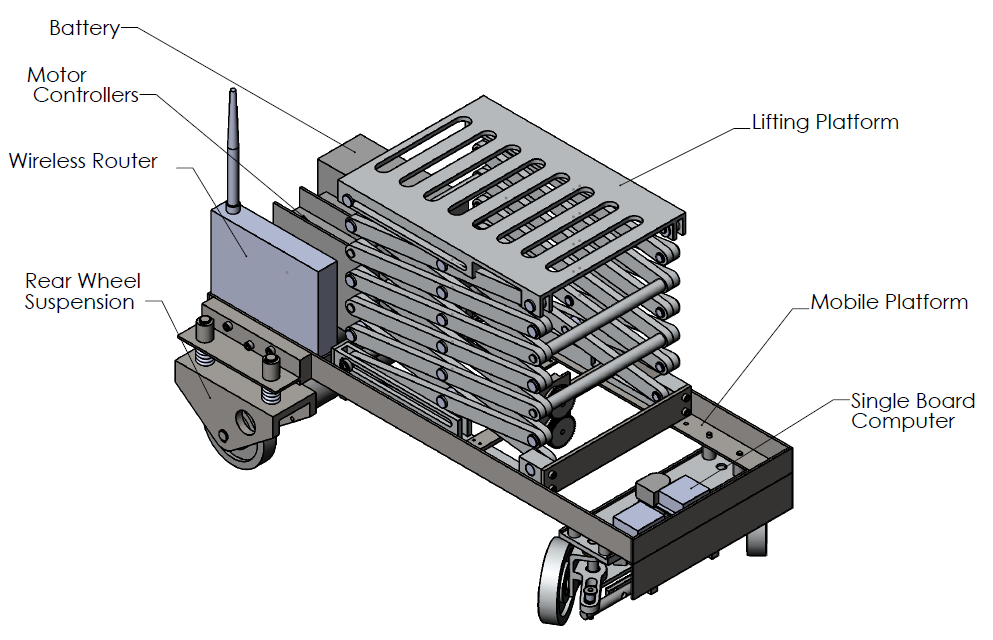
\includegraphics[height=5cm,keepaspectratio]{Chapter3/fig/robo3Dmodel}
% 		\captionof{figure}{3-D Model of the mobile manipulator}
% 		\label{fig:robo3Dmodel}
% 	\end{minipage}%
% 	\begin{minipage}{.5\textwidth}
% 		\centering
% 		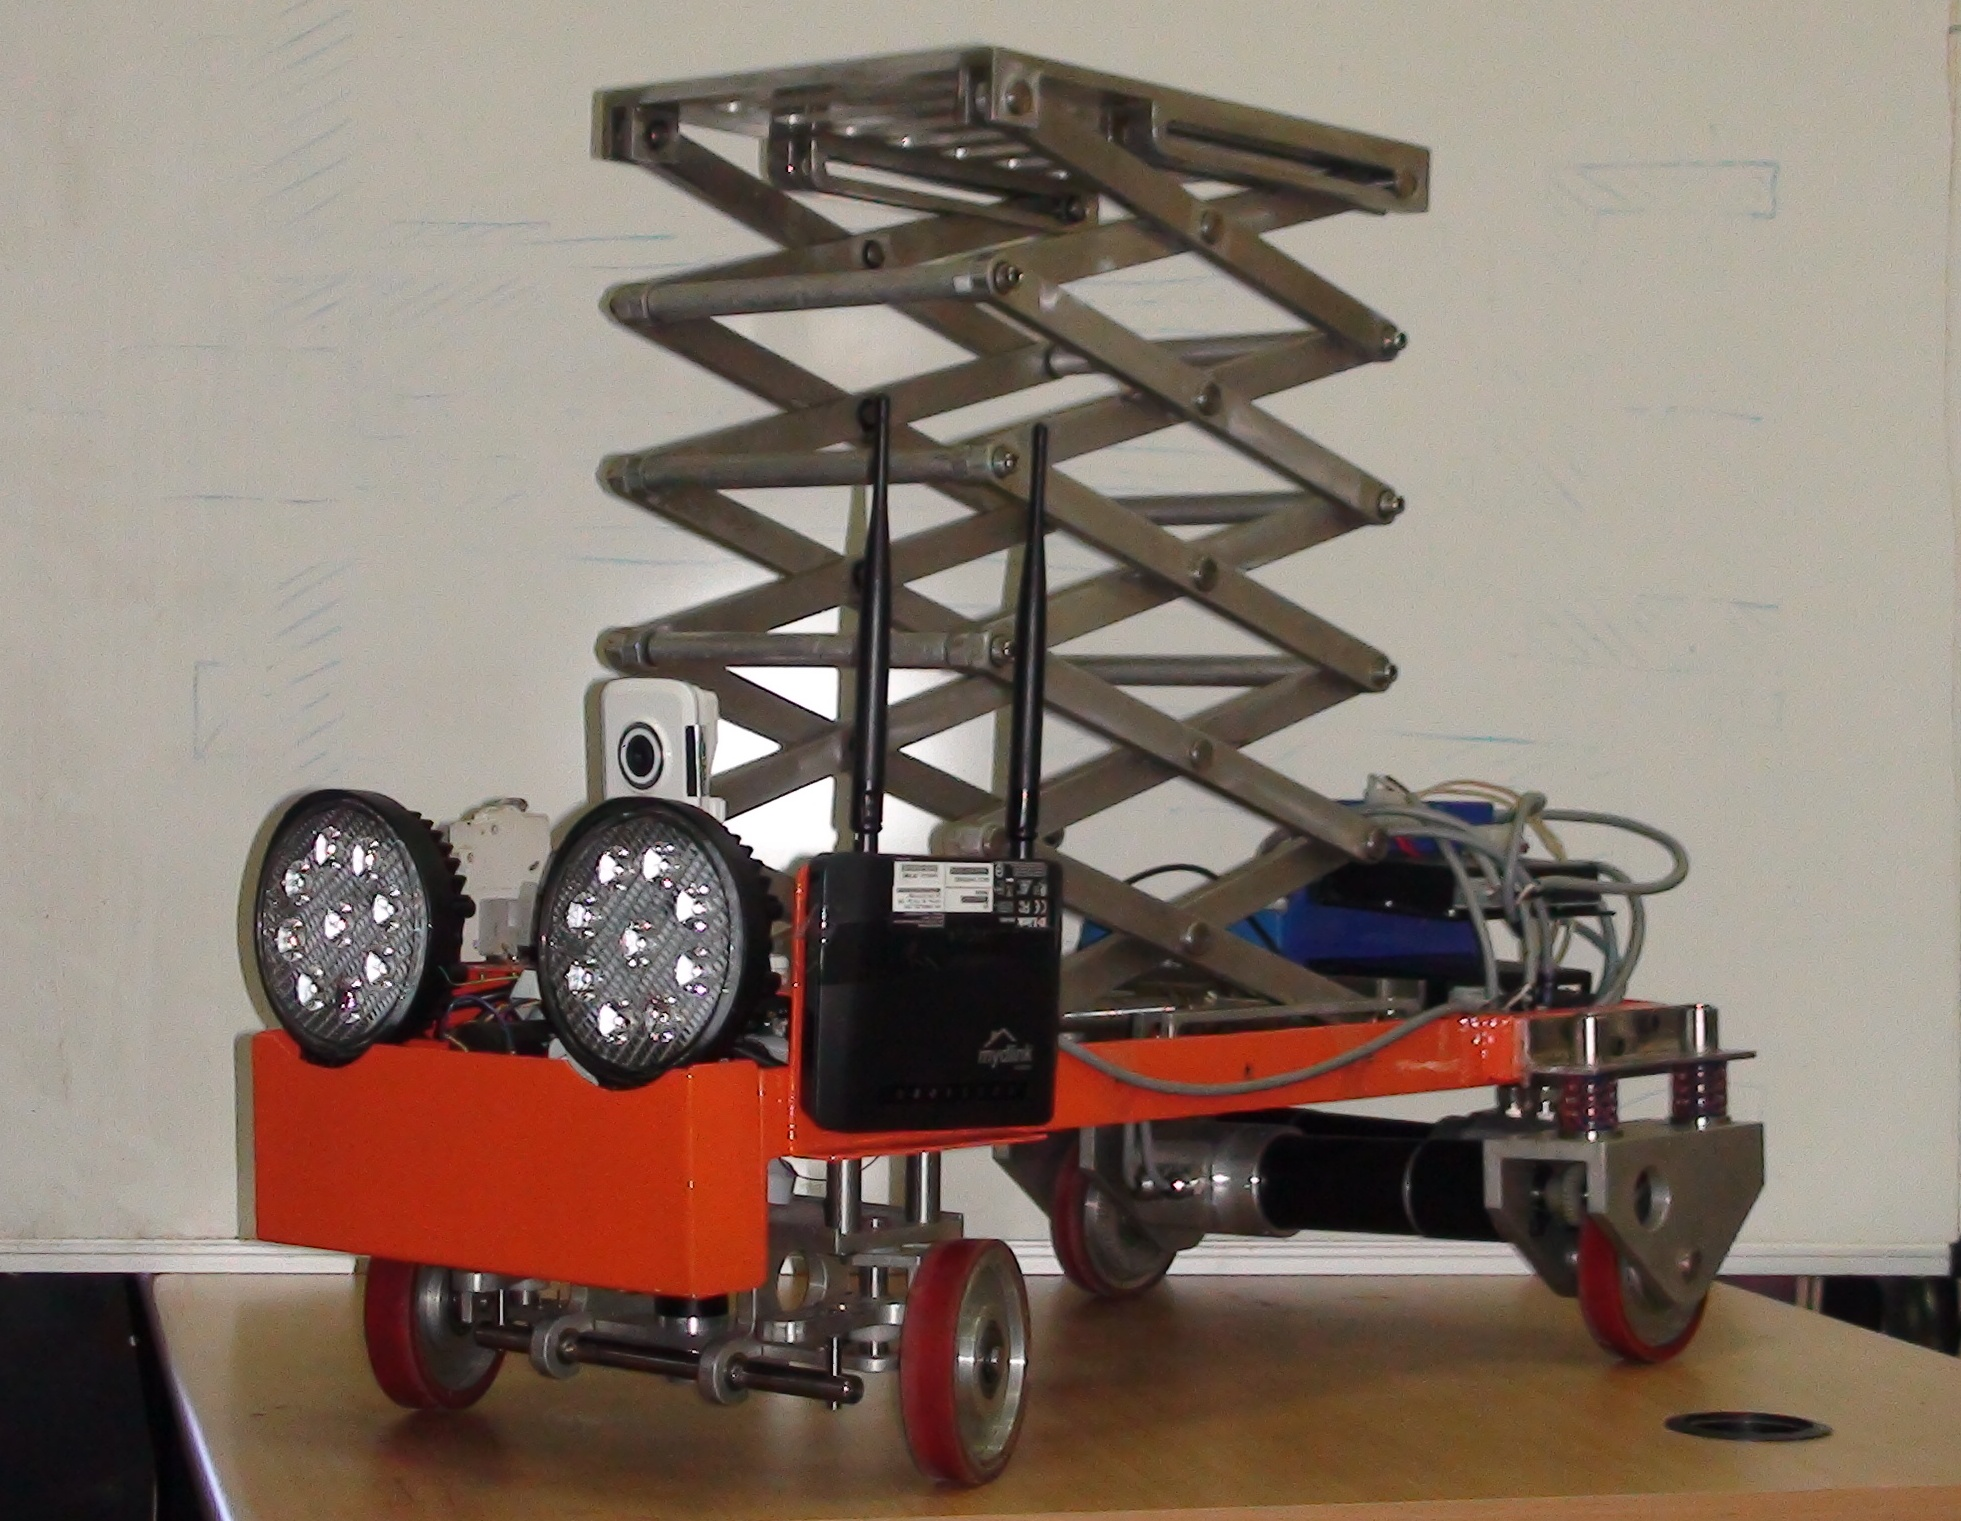
\includegraphics[width=.8\linewidth,height=5cm,keepaspectratio]{Chapter3/fig/roboActual}
% 		\captionof{figure}{Photograph of the actual System}
% 		\label{fig:roboActual}
% 	\end{minipage}
% \end{figure}

%
\begin{table}[!htbp]
	\caption{Key parameters and specifications of the mobile manipulator.}
	\label{tb:specifications}
	\centering
	\begin{tabular}{l l l}
		\hline
		
		%\emph{Parameter}  & \emph{Example} & \emph{Font size and style} \\
		%\hline
		Weight  & 70 Kg & Without payload \\ 
		Payload & 10 Kg &---\\
		Footprint & 700 mm $\times$  400 mm & - \\
		Height Collapsed & 500 mm  & Along  Z-Axis\\
		Height Extended & 1500 mm & Along  Z-Axis  \\
		Steering mechanism & Davis Steering & --\\
		Turning radius & 415 mm & - \\
		Ground clarence & 45 mm & --\\
		Maximum traction speed & 30 m/min & On flat terrain \\
		Ramp climb angle & $30^\circ $ & Platform in retracted position\\
		\hline
	\end{tabular}
\end{table}

The mobile manipulator has a footprint of 700 mm $\times$  400 mm  based on the narrow passage through which the system  has to negotiate. These passages are formed inside the vault area by the pipelines and  structural supports of the cyclotron and its associated equipment.  Two DC motors, with speed servo controller,  provide the traction to each rear wheels. The two front wheels are  inter-connected with a Davis steering mechanism \cite{TOMBook}. A scissor mechanism provides the vertical  motion to the detector that is mounted on the manipulating arm.

 In order to keep the self weight of the system small, all the  structural parts are made of aluminum alloy AL6061, apart from the base frame. Stainless Steel (SS304)  angle sections was used for the base frame, which give it  excellent strength to weight ratio. 
 
 \section{Kinematic Topology}
 \label{sec:KineTopo}
 One of the major requirements of the proposed mobile manipulator was that it should be tolerant to single actuator failure, as mentioned in  Chapter 1. The objective was to increases the reliability of the robotic platform. The second major objective was easy and intuitive manoeuvrability  of the platform under teleopration.
 
 The robot has four wheels arranged in a rectangular configuration. This provides  more stability as the support polygon is large with respect to other configuration such as rhombus. The rectangular wheel position layout has another advantage that it is car like, which makes driving intuitive. 
  
  The proposed mobile manipulator has two rear wheel  driven by two independent motors.  The front wheels are passive wheels, steered by a single motor connected through Davis Steering linkage. Thus the total no of actuators used by the mobile platform is three.
 
 This kinematic topology of the RARS robotic platform makes it tolerant to single actuator failure. In case the steering actuator fails, the RARS can be operated as a differential drive robot. The system still has all the required mobility (2-DOF) to bring it to any desired location.
 
 In case one of the rear wheel drive motor fails, it becomes kinematically similar to the bicycle model \cite{campion1996structural}. The system is still a 2-DOF system. It can be operated in this mode to bring to any desired location.
     

\section{Design of the Traction System}
Traction is provided by the two rear wheels driven independently. This makes the system over actuated. A mechanical differential connecting the two rear wheels, as used in cars,  would overcome this. It was not proposed to do so as the proposed vehicle is planned to be teleoperated in a environment inaccessible to humans. This calls for a single-failure-safe design. The proposed design gives two major advantages. 
Firstly, in case  one of the wheel loosing contact with the ground due to  overhang in small pits or while over an obstacle, the mechanical differential system would keep supplying power to the free hanging wheel. The system will hence get stuck, maybe in an unrecoverable location. This situation is avoided in the present design as the motor having traction can be independently powered, to move the vehicle.  
Secondly, using the proposed design, in case of one  actuator failure, either the traction or the steering motor, still the vehicle can be manoeuvred to a  safe location, albeit with dragging of the wheel with failed actuator.

 \begin{figure}[h]
	\centering
	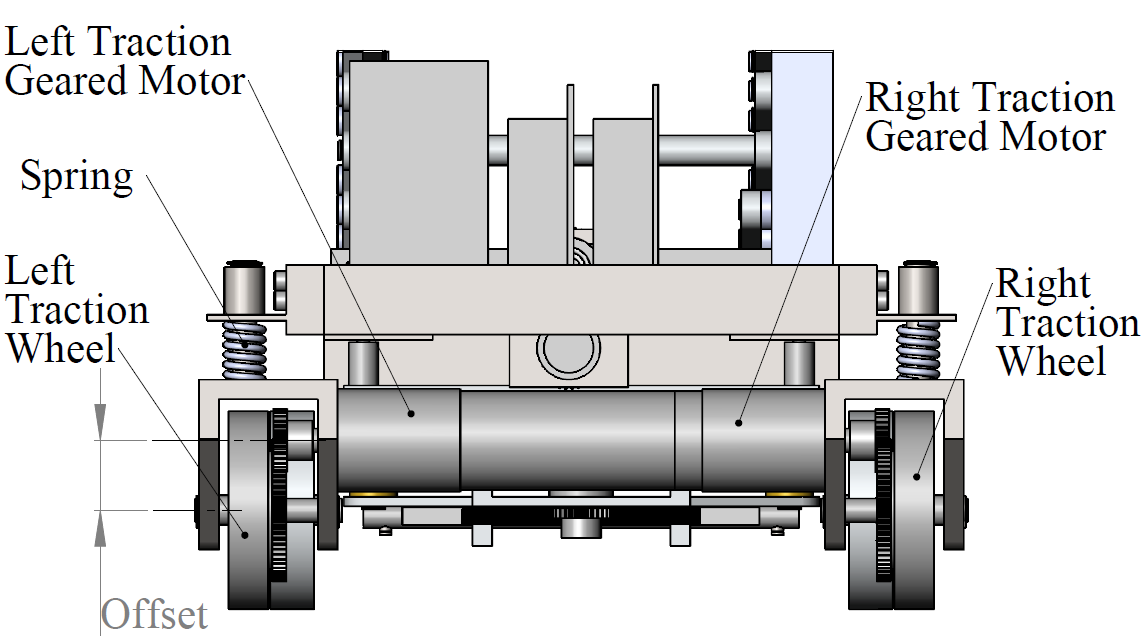
\includegraphics[width=.7\linewidth,keepaspectratio]{Chapter3/fig/WheelOffset}
	\captionof{figure}{Rear suspension}
	\label{fig:tractionDrive}
\end{figure}

    Each wheel is driven by a  Maxon DC RE50 200W Motor through a 26:1 reduction gearbox. The motors are mounted at an offset to the wheel axis for increased ground clearance and lateral compactness, as shown in Figure \ref{fig:tractionDrive}. Spring suspension is provided at each wheel to ensure sufficient contact force on uneven  ground. The diameter of the wheel is 100 mm $(D_w)$, which is sufficient to ride over obstacle of height 20 mm (Max). They are made of Aluminum alloy-6061 with 5mm thick molded polyurethane (PU) liner. The PU liner provides large traction on cement flooring while being resistant to wear.
    
   \begin{figure}[h]
   	\centering
   	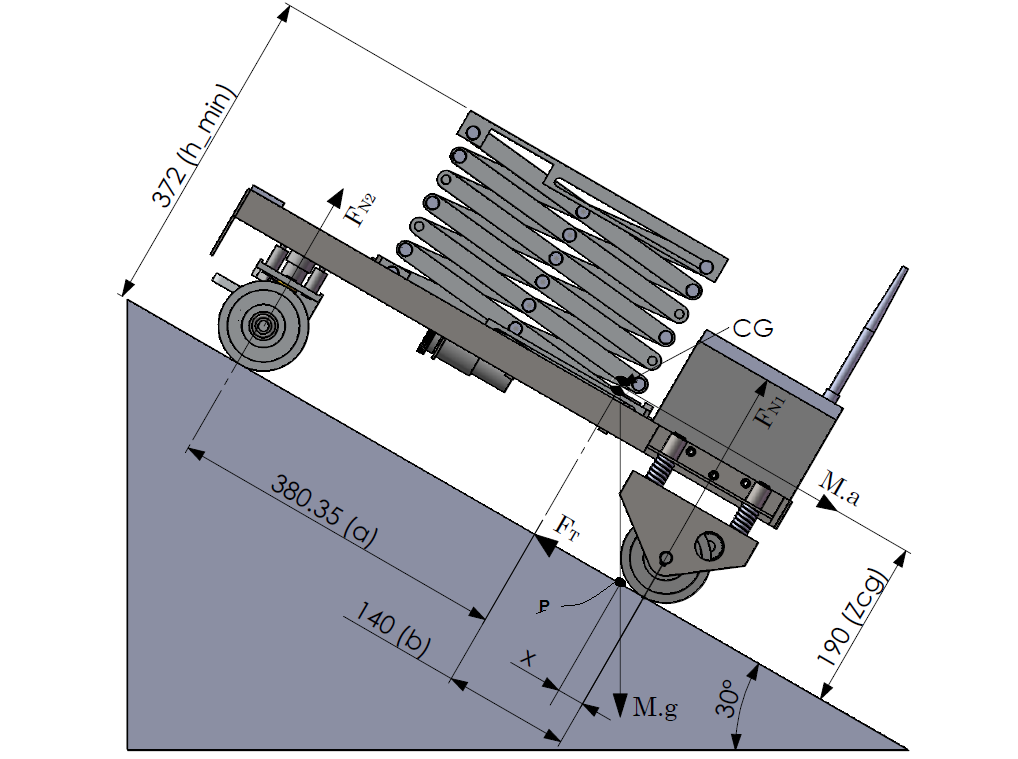
\includegraphics[width=0.85\linewidth,keepaspectratio]{Chapter3/fig/loadDist}
   	\captionof{figure}{Mobile manipulator on slope}
   	\label{fig:loadDistribution}
   \end{figure}
\subsection{Stability of mobile manipulator}
One of the methods to study stability of dynamic structure is to use \textit{Zero Moment Point} or ZMP introduced by Vukobratovic et al. \cite{vukobratovic1969contribution,vukobratovic2012biped}. It was used for stability analysis of mobile robots as discussed in the literature survey section of this thesis.
The idea of ZMP-stabilization  is to find a point on the ground where the net  moment due to all forces acting on the mobile manipulators is zero. This point is called the ZMP. If the ZMP is inside the \textit{support polygon} then the system is stable. A support polygon is a convex polygon formed by joining points of contact of the mobile robot with the ground. The support polygon for the RARS robot is given by $\{O_1,O_2,O_4,O_5\}$ as shown in Figure \ref{fig:supportPoly}. To make the analysis simpler and conservative we will use the rectangular polygon formed by $\{A, B,O_4,O_5\}$ shown by black hash in Figure \ref{fig:supportPoly}. 


  The two major forces action on a dynamic system is the gravitational force and the inertial forces due to acceleration. They all act at centre of mass of the robot. Therefore the distribution of load becomes very important. From stability point of view the center of mass should be centrally located in the support polygon $\{A, B,O_4,O_5\}$ , whereas to generate maximum traction the CG should be close to rear wheel axel, i.e., on side AB  of the support polygon. 
  The load distribution was optimized to generate maximum normal reaction, $F_n$,  at the rear wheels without overturning while moving up the ramp of $30^o$ with the manipulator in the collapsed condition as shown in Figure  \ref{fig:loadDistribution}. Maximizing rear wheel reaction by increasing $b$, as per Equation \ref{eqn:loadratio} ensures increased traction, $F_T=\mu F_N$ ($\mu$ is the coefficient of friction), but at the same time decreases the stability margin indicated by ``x" in Figure \ref{fig:loadDistribution}.
  \begin{equation}
  \label{eqn:loadratio}
  F_{N2}=\frac{m_rg\cos\theta}{a+\frac{1}{b}}
  \end{equation}
  Let $p$, be the position ZMP located at a distance $x$ form the rear wheel contact point, then we get
  \begin{equation}
  \label{eqn:zmpRARS}
  x(F_{N2}-m_r g \cos \theta+F_{N1})=(a+b)F_{N2}+ m_r (a_l +g \sin \theta )z_{cg} -m_r g b \cos\theta
  \end{equation}
   Assuming that the \textit{ZMP}, is at the rear wheel contact point, i.e., $x=0$ the above equation reduces to
\begin{equation}
\label{eqn:zmpRear}
(a+b)F_{N2}=b(m_r g\cos\theta)-z_{cg}(m_r g\sin\theta+m_r a_l)
\end{equation}
The critical condition,which  initiates over turning about the rear axle is given by $F_{N2} =0$.  This reduces the above equation \ref{eqn:zmpRear} to 
\begin{equation}
\label{eqn:overturn}
m_rgb\cos\theta=(m_rg\sin\theta+m_r \bar a)z_{cg}, \quad \Rightarrow g(\frac{b}{z_{cg}}\cos\theta-\sin\theta)= a_l
\end{equation}

 

where 
\begin{itemize}
\item[] $F_{N1}$, $F_{N2}$ :  normal reaction on the front and rear wheels.
\item [] $ a_l$ : the linear acceleration of the mobile robot along the ramp.
\item[] $a$ and $b$ :  the distance of the vehicle centre of gravity (CG) from the rear and front wheels.
\item [] $Z_{cg}$ :  the height of  CG from the  plane containing the contact point of the wheels.
\item [] $m_r$ : mass of the vehicle.
\item [] $g$ : acceleration due to gravity.
\item[] $\theta$ :  the inclination of the traction surface from horizontal.
\end{itemize}
The mass distribution of the mobile robot was  adjusted such that the stability margin $x$ as shown in Figure \ref{fig:loadDistribution} was fixed to $30$ mm, which  limits  the acceleration of the mobile robot while climbing up  over a ramp of $30^o$ to $ a_l=0.144g$. Operation of system below this acceleration limit safeguards it against overturning along the longitudinal direction. 

The stability analysis of the RARS robot on a ramp  was carried out with the manipulator in the retracted condition. In case the manipulator is extended  the CG of the system shift towards the rear wheel axle. A condition will be reached when the vector $Mg$ crosses the rear wheel contact point, and the mobile robot will overturn. To insure against this unstable situation the vehicle is never moved on the ramp with manipulator extended.
   
Another instability is encountered during turning or negotiating the curve. The centrifugal force tends to overturn the vehicle in lateral direction as shown in Figure \ref{fig:LatOverturn}.
If $p$ is the ZMP for this configuration, the location of ZMP, i.e., $x$ is given by Equation \ref{eqn:zmp2}. 
\begin{equation}
\label{eqn:zmp2}
2dN_3+ \frac{m_r v^2}{R}-m_r g d=x(N_4+N_3-M_r g)
\end{equation}
The overturning will start when ZMP reaches the outer boundary of the support polygon that is on the side $O_4B$ or $O_3A$ and $N_3$ or $N_4$ becomes zero respectively.
This limits the linear velocity of the vehicle for a given steer angle. If $v$ is the linear velocity of the vehicle and $R$ the radius of the path, if the above overturning conditions i.e., $x=0$ and $N_3=0$  are applied to the above equation, we get

\begin{equation}
\label{eqn:LatOverturn}
\frac{m_r v^2}{R}Z_{cg}=m_r g d 
\end{equation}
Thus the limiting velocity as a function of $R$  (turning radius)
\begin{equation}
\label{eqn:Vel_limit}
v=\sqrt{\frac{R g d}{Z_{cg}}}
\end{equation}
This sets the limiting velocity as $v=1.9$ m/sec based on the $Z_{cg}=190$ mm and $d=168$ mm as shown in  Figure \ref{fig:loadDistribution} and \ref{fig:LatOverturn}. Where, R equals the minimum turning radius of the vehicle which is $415$ mm as given in Table \ref{tb:specifications}.

\begin{figure}
 	\centering
 	\begin{minipage}{.5\textwidth}
 		\centering
 		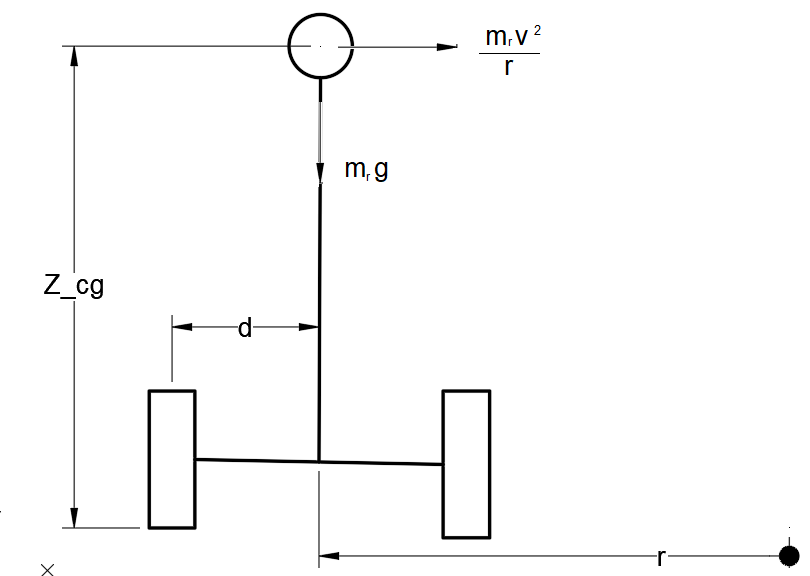
\includegraphics[width=.9\linewidth,height=4.5cm,keepaspectratio]{Chapter3/fig/LateralOverturn}
 		\captionof{figure}{Centrifugal forces}
 		\label{fig:LatOverturn}
 	\end{minipage}%
 	\begin{minipage}{.5\textwidth}
 		\centering
 		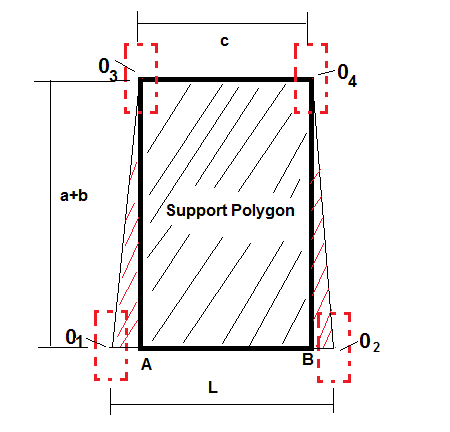
\includegraphics[height=5cm,keepaspectratio]{Chapter3/fig/Supportpolygon.png}
 		\captionof{figure}{RARS support polygon}
 		\label{fig:supportPoly}
 	\end{minipage}
 \end{figure}

 \subsection {Selection of motor and gearbox}
 The torque requirement for the rear wheels were calculated based on the static moment balance with the assumption that each rear wheel shares equal load and the total suspended weight is 80 kg. From the freebody diagram (Figure   \ref{fig:loadDistribution}), using moment and force balance  we get the following:
\begin{equation}
\label{eqn:t1}
F_{N1}=\frac{a M \cos \theta}{a+b-\mu Z_{cg}} , \quad \quad
F_T=\mu F_{N1}
\end{equation}
In order to estimate the traction motor size, we take worst case scenario of $\theta=30^o$ and $\mu =0.3$. This leads to
\begin{equation*}
F_{N1}=66 \text{ kg}, \quad\quad F_T=0.3\times 66 \approx 20 \text{ kg}
\end{equation*}
 Since the traction is provided by the two rear wheels, the torque required per wheel $(T_w)$ is given by
\begin{eqnarray}
T_w=(F_T/2)(D_w/2)= (20/2) \times 50=500 \text{ Kg-mm } \simeq 5 \text{ Nm}
\end{eqnarray}
The motor torque $T_M$, required based on the assumption of factor of safety, $FS=1.5$ is
\begin{equation}
T_M=(FS)\times T_w=1.5\times 5 =7.5 \simeq 8 \text{ Nm}
\end{equation}
 Assuming the maximum speed, $V_{ramp}=1$ m/s, of the mobile manipulator over a ramp, the required power, $P_M$, of the traction motor is calculated as,
 \begin{equation}
 \begin{aligned}
\omega_w&=V_{ramp}/(D_w/2) \simeq 200 \text{ rpm}\\
P_m&=\omega_w T_m=20\times 8=160 \text{ W}
 \end{aligned}
 \end{equation}
 The nearest Maxon motor available as per the catalogue \cite{catMaxon} is 200 W,  RE50-370354 motor.  The nominal speed, $N_s$ is 5680 rpm. Therefore, the  gearing  ratio required is, $N_s/\omega_w=5680/200 \simeq 28.4$. The nearest gear box available  is of ratio $26:1$, which was chosen. 

\section{Design of Steering System }
The design objective of a steering system should be to ensure rolling motion of all the  wheels during every possible manurers of the mobile robot. This is  to reduce the friction drag due to sliding motion which degrades the energy efficiency of a mobile robot. In case of four wheeled vehicle, with the orientation of the rear wheels fixed and front wheels steered, the condition   shown in Figure \ref{fig:steerCond},  referred in some literature as Ackerman steering condition, must be satisfied to ensure pure rolling of all the wheels.   

This mobile manipulator uses Davis steering mechanism,  Figure \ref{fig:davis},  on the front wheels. Caster wheels  were not used as they tend to align with  obstacles and thus get stuck. On the  other hand tracked wheels have excellent rough terrain capabilities, but is power intensive due to skid steering. Another option was to use   Omnidirectional wheels, which need complex controller for coordination and an extra actuator. Moreover, the  floor of the cyclotron are  in general not clean of loose small objects, which may get stuck in between the free rollers of the omnidirectional wheels. This will reduce the efficiency of the vehicle.  

\begin{figure}
 	\centering
	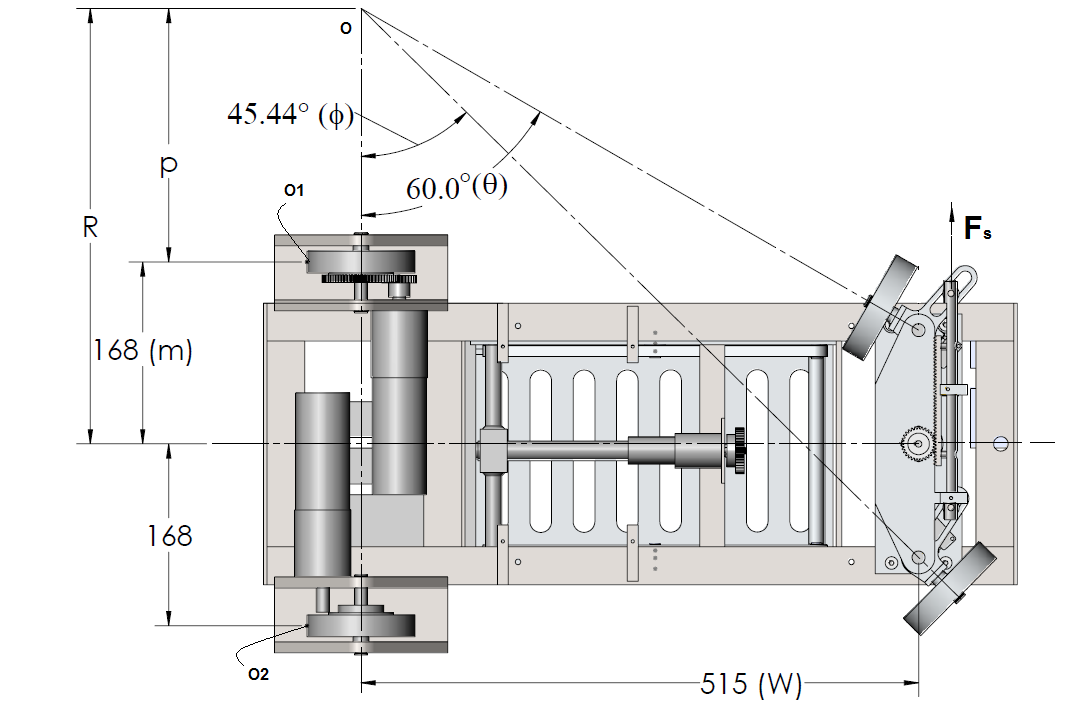
\includegraphics[width=\linewidth,keepaspectratio]{Chapter3/fig/steerringCondition}
	\captionof{figure}{Ackerman steering condition }
	\label{fig:steerCond} 
\end{figure} 
 

Davis steering mechanism was chosen over Ackerman steering gear as it satisfies the steering condition given by  Equation \ref{eqn:Acker}, which ensures pure rolling of all  wheels, over the entire steering range. This makes the system, suitable for passive wheel odometry and also energy efficient.  The steering gear being positively driven by position controlled servo motor does not align with the obstacles and thus are able to crossover it. The dimensions of the links used in the steering mechanism is given in Figure \ref{fig:davis}, and are based on the Ackerman steering law given below:
\begin{equation}
\label{eqn:Acker}
\cot\phi-\cot\theta=a/w, \quad  \frac{2b}{h}=\frac{a}{w}
\end{equation}
where $a$ and $b$ is limited by the overall size of the vehicle, discussed earlier.

\subsection{Minimum turning radius}
The mechanical construction of this steering mechanism limits the steering angle. This in turn limits the minimum radius the vehicle can negotiate. The parameters of the steering linkages were found using  optimization with constraints on overall dimensions and location  of links. The details of the method used is given in Appendix \ref{Ch:ApenC}. The
Figure \ref{fig:steerCond} shows the extreme values of $\phi$ and $ \theta$, one side of the steering limits. The \textbf{ turning radius } $R$ for a given steer angle $\theta$  is calculated  from the geometry of Figure  \ref{fig:davis} as
\begin{equation*}
\tan\theta =\frac{w}{p+m-\frac{a}{2}} \quad \text{and} \quad R=m+p
\end{equation*}
Eliminating $p$  from the above equation and rearranging , we get 
\begin{equation}
\label{eqn:turningRadius}
R(\theta)=\frac{a}{2}+w\cot\theta
\end{equation}
The extreme value of $\theta=60^o$ as shown in Figure \ref{fig:steerCond}, this gives the \textit{minimum turning radius } $R_{min}$ as
\begin{equation*}
R_{min}=\frac{210}{2}+515  \cot(60^o)=402~\text{mm}
\end{equation*}

\begin{figure}
	\centering
	\begin{minipage}{.5\textwidth}
		\centering
		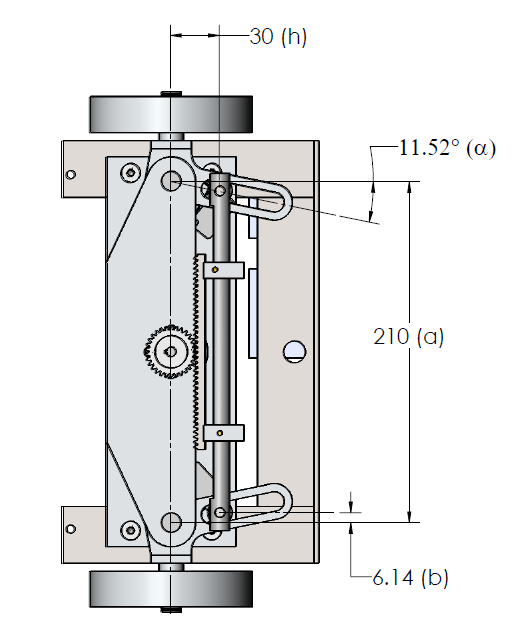
\includegraphics[width=\linewidth,height=6.5cm,keepaspectratio]{Chapter3/fig/davis}
		\captionof{figure}{Davis steering gear}
		\label{fig:davis}
	\end{minipage}%
	\begin{minipage}{.5\textwidth}
		\centering
		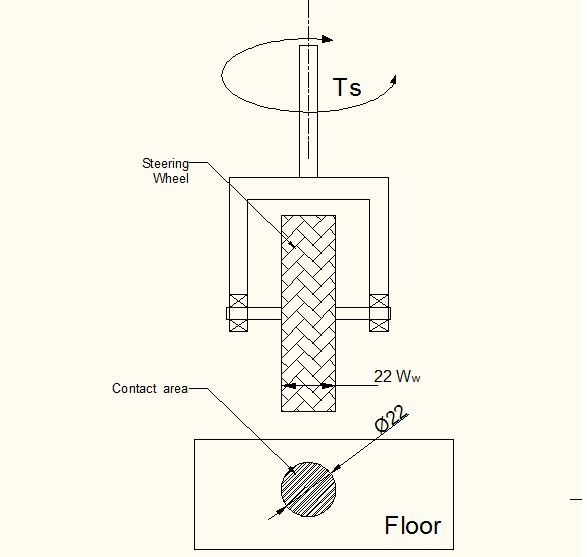
\includegraphics[width=\linewidth,height=6.5cm,keepaspectratio]{Chapter3/fig/steerTorqCal}
		\captionof{figure}{Steer torque}
		\label{fig:steerTorq}
	\end{minipage}	
\end{figure} 

\subsection{Calculation of steering torque}
\label{sec:SteerinTorqueStatic}
In order to choose an appropriate steering motor some torque estimate was needed, which is carried out in this section. 
The torque required to steer the front wheel is estimated based on static equilibrium because the system moves at very slow speed (0.5 m/sec). A simplified assumption was made that the wheel deforms under normal load and the contact area thus generated is  circular in shape with diameter that of the wheel width, $W_w$, as shown in Figure \ref{fig:steerTorq}. 
In order to estimate the normal reaction on each wheel, we assumed that the total weight of 80kg was equally shared by the four wheels. 
Therefore, $N_s=80/4=20$ kg. Next, the uniform pressure formula \cite{TOMBook} used for  brakes/clutches design was applied to find the resistance  torque $T_s$, between the ground and the wheel i.e., 
\begin{equation}
\label{eqn:brake}
T_s=\frac{N_s\mu}{3}W_w= 0.4~\text{Nm}
\end{equation}  
The resistance torque, $T_s$, of  both the wheels  are balanced by the force $F_s$ acting on the rack as shown in Figure \ref{fig:steerCond}. The rack is coupled to the steering motor by a pinion of diameter, $D_p=40$ mm. The motor  torque, $T_{m_s}$  in Equation  \ref{eqn:SteerTq} is calculated with a  high factor of safety, $FS=3$. This is because $T_S$ is estimated  based on a simplified model of brake design. The power, $P_{m_s}$ of the steering motor based on  torque $T_{m_s}$ and the steering speed $\omega_s$ of 100  rpm is 
\begin{equation}
\begin{aligned}
\label{eqn:SteerTq}
T_{m_s}=(FS)\frac{2T_s}{h}\frac{D_p}{2}=1.6\text{ Nm} \quad \text{and}\quad P_{m_s}=T_{m_s}\omega_s=17\text{ W}
\end{aligned}
\end{equation} 

Based on the above specifications, a 20W, RE25 DC motor of Maxon  make and a gear box  GP32 of ratio 159:1 was chosen for the steering mechanism. 
 
\section{Scissor Mechanism for Manipulator Arm}
 The manipulating arm  was designed to move  the radiation sensor mounted on the \textit{``lifting platform"} up to a height of 1.5 m from the floor level. This motion was generated using  a scissor mechanism,  shown in Figure \ref{fig:scissor}. The scissor mechanism has two major advantages over other lifting methods such as telescopic pillar, screw or belt based linear motion units, etc.  First, the  ratio of height in extended and collapsed condition is very large. In our case it is $3:1$. Second, the self weight of the mechanism is less as it is made of links having rectangular cross-section.

The scissor mechanism, Figure \ref{fig:scissor}, has 6 stages, where each ``X" denotes one stage. 
\begin{figure}
	\centering
	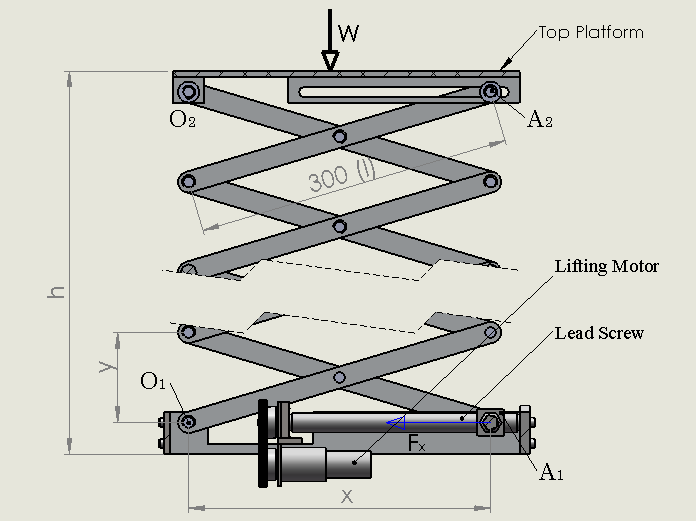
\includegraphics[width=.8\linewidth,keepaspectratio]{Chapter3/fig/scissor}
	\captionof{figure}{Scissor mechanism}
	\label{fig:scissor}
\end{figure}
The Scissor is connected to the top platform by a pivot joint $O_2$ and a prismatic joint $ A_2$, and coupled to the base frame by pivot joint $O_1$ and a prismatic joint $A_1$. The linear actuation of joint $A_1$ is provided by a lead screw of pitch ($P$) 1.5 mm and mean diameter ($d_m$) 10 mm.  This results in vertical motion of the top platform. 
  
 The relation between the vertical motion of the platform and the horizontal displacement of point $A_1$ is given by geometry of the mechanism shown in Figure \ref{fig:scissor} 
\begin{equation}
\begin{aligned}
y&=l\sin\theta\;\quad \Rightarrow dy=l\cos\theta d\theta;\\
 x&=l\cos\theta \; \quad \Rightarrow dx=-l\sin\theta d\theta\\
h&=Ny~~~\; \quad\Rightarrow dh=Ndy
\end{aligned}
\end{equation} 
where, $l$ is the link length, $\theta$ the angle of the link with horizontal plane, $N$ the number of stages, and $h$ the height of platform.


The number of stages used in the scissor mechanism is six (N=6). From the principle of virtual work, we get 
\begin{equation}
\label{eqn:ScissorForce}
\begin{aligned}
-F_xdx=Wdh,\;\Rightarrow F_x=\frac{WN}{\tan\theta}
\end{aligned}
\end{equation}
where, $F_x$ is the axial force on the prismatic joint, $A_1$, and W is the payload. From Equation \ref{eqn:ScissorForce}, it is clear that as $\theta\rightarrow 0$, the force  $F_x \rightarrow \infty$. In the present design,  $\theta_{min}=5^o$ and $\theta_{max}=45^o$. Therefore, the extended height  $h_{max}=Nl\sin\theta_{max}=1.3~$m and the collapsed height $h_{min}=156~$mm. Assuming $W=8~$kg as payload the maximum force $F_x=342~$kg is required at $\theta_{min}=5^o$, . 

The motor torque required for the scissor mechanism is calculated using  screw jack formula given in  \cite{TOMBook} and  presented here as Equation \ref{eqn:liftingTorque}. 
\begin{equation}
\label{eqn:liftingTorque}
\begin{aligned}
T_L&=\frac{F_x d_m}{2}(\frac{p+\pi\mu d_m\sec\alpha}{\pi d_m-\mu p\sec \alpha})=7.5\text{ Nm}
\end{aligned}
\end{equation}
where coefficient of friction, $\mu=0.1$, ACME thread angle, $2\alpha=60^o$, pitch diameter, $d_m=15$ mm, and pitch, $p=1.5$ mm, is used. Based on the above specification $10~$W, RE20 DC motor with a gear box of 25:1 ratio was chosen from Maxon motor catalogue ~\cite{catMaxon}.



  
  

\section{Summary}
A customized design of a mobile manipulator taking into consideration the field requirements and floor condition existing inside the cyclotron vault is presented. Requirement of an overactuated system and the advantage  of the proposed kinematic design over other redundantly actuated system is discussed. The advantage of scissor mechanism for vertical motion of the sensor over other mechanism is highlighted.
Design calculations for motor selection and stability analysis using ZMP to arrive at the maximum permitted acceleration for the proposed  RARS mobile manipulator are presented. 

 


